\hypertarget{ux8d21ux732eux8005}{%
\subsubsection{贡献者}\label{ux8d21ux732eux8005}}

问题:谁是项目的贡献者?

\hypertarget{ux63cfux8ff0}{%
\paragraph{描述}\label{ux63cfux8ff0}}

贡献者是指以任意方式为项目做出贡献的人。
这一指标确保所有类型的贡献在项目中都能得到充分认可。

\hypertarget{ux76eeux6807}{%
\paragraph{目标}\label{ux76eeux6807}}

开源项目由许多贡献者组成。
认识项目的所有贡献者对于了解个人参与的活动非常重要,比如谁在帮助代码开发、事件规划和营销工作等。

\hypertarget{ux5b9eux73b0}{%
\paragraph{实现}\label{ux5b9eux73b0}}

从项目使用的协作工具中收集作者姓名。

\textbf{聚合器:}

\begin{itemize}
\tightlist
\item
  计数。 给定时间内的贡献者总数。
\end{itemize}

\textbf{参数:}

\begin{itemize}
\tightlist
\item
  时间段。 开始日期和完成日期。 默认:永久。 计算贡献的时期段。
\end{itemize}

\hypertarget{ux7b5bux9009ux6761ux4ef6}{%
\subparagraph{筛选条件}\label{ux7b5bux9009ux6761ux4ef6}}

按参与地点。 例如:

\begin{itemize}
\tightlist
\item
  提交作者
\item
  议题作者
\item
  审查参与者,例如拉取请求中
\item
  邮件列表作者
\item
  事件参与者
\item
  IRC 作者
\item
  博客作者
\item
  按发布周期
\item
  项目活动的时间框架,例如,寻找新贡献者
\item
  项目的编程语言
\item
  项目中的角色或职能
\end{itemize}

\hypertarget{ux53efux89c6ux5316ux6548ux679c}{%
\subparagraph{可视化效果}\label{ux53efux89c6ux5316ux6548ux679c}}

\begin{enumerate}
\def\labelenumi{\arabic{enumi}.}
\item
  贡献者名称列表(通常带有参与程度的信息)

  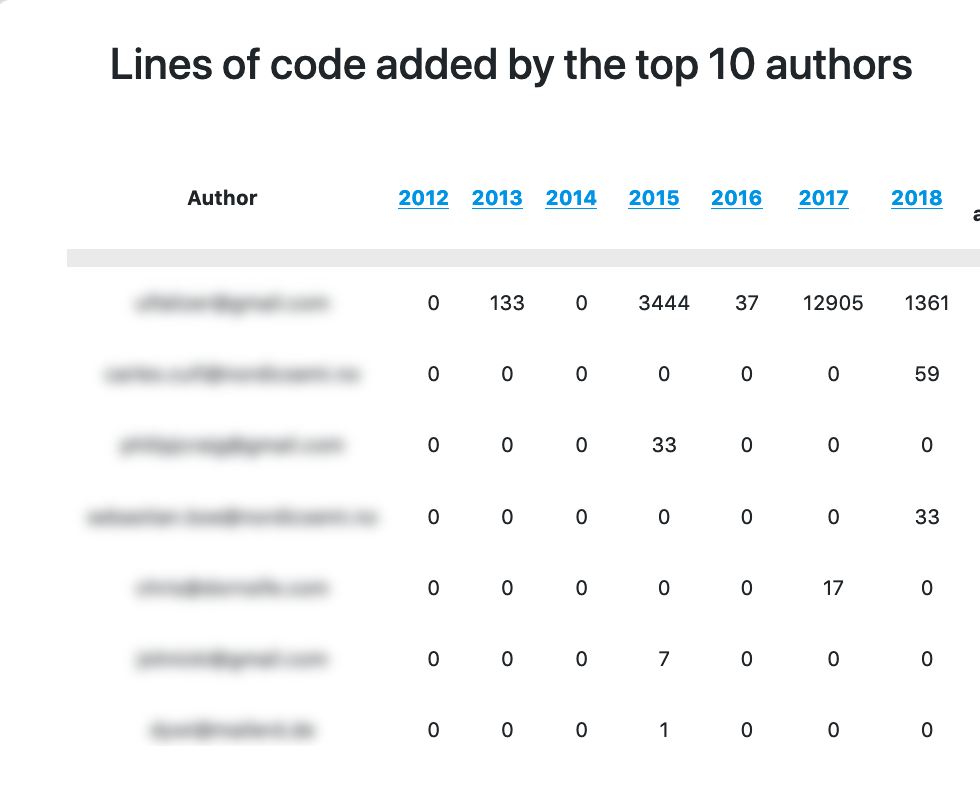
\includegraphics{images/contributors_top-contributor-info.png}
\item
  贡献者人数汇总

  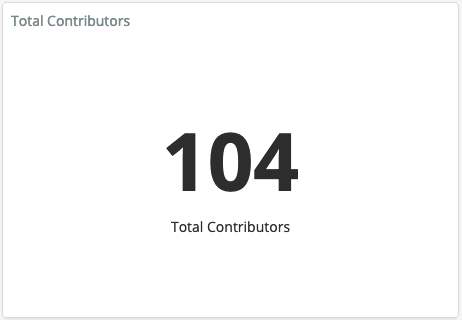
\includegraphics{images/contributors_summary-contributor-number.png}
\item
  活跃贡献者数量随时间的变化
\end{enumerate}

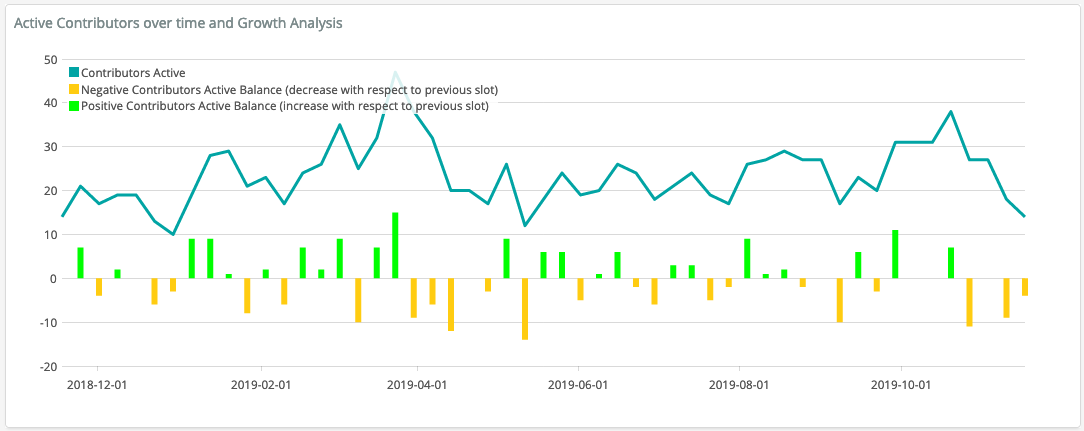
\includegraphics{images/contributors_growth.png}

\begin{enumerate}
\def\labelenumi{\arabic{enumi}.}
\setcounter{enumi}{3}
\tightlist
\item
  新贡献者(按首次贡献日期对贡献者排序)
\end{enumerate}

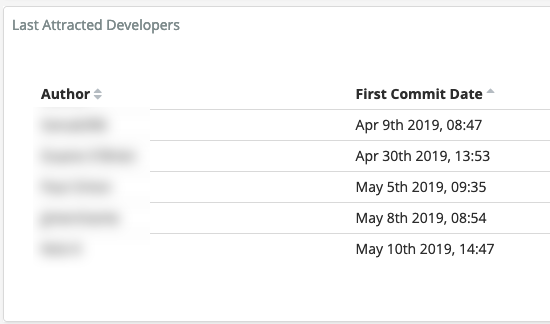
\includegraphics{images/contributors_first-commit-date.png}

\hypertarget{ux63d0ux4f9bux6307ux6807ux7684ux5de5ux5177}{%
\subparagraph{提供指标的工具}\label{ux63d0ux4f9bux6307ux6807ux7684ux5de5ux5177}}

\begin{itemize}
\tightlist
\item
  \href{https://chaoss.github.io/grimoirelab/}{GrimoireLab}
\item
  \href{http://augur.osshealth.io/api_docs/\#api-Evolution-Contributors_Repo_}{Augur}
\end{itemize}

\hypertarget{ux6570ux636eux6536ux96c6ux7b56ux7565}{%
\subparagraph{数据收集策略}\label{ux6570ux636eux6536ux96c6ux7b56ux7565}}

如上所述,部分贡献者信息可以通过 GrimoireLab 和 Augur 等软件获得。
然而,有些贡献者洞察不太容易通过跟踪数据获得。
在这些情况下,使用社区成员调查或事件注册的方式可以提供所需信息。
示例问题包括:

\begin{itemize}
\tightlist
\item
  采访问题:通常哪些贡献者不会出现在贡献者列表中?
\item
  采访问题:哪些贡献者经常不被视为重要贡献者,因为其贡献更倾向于``幕后''?
\item
  采访问题:您经常与哪些社区成员合作?
\end{itemize}

此外,社区成员调查可以提供有关项目贡献的更多信息。 示例问题包括:

\begin{itemize}
\tightlist
\item
  李克特量表 {[}1-x{]} 项:我正在为项目做贡献
\item
  矩阵调查项:您在项目中多久参与一次以下活动?

  \begin{itemize}
  \tightlist
  \item
    列标题:从不,很少(每月少于一次),有时(每月一次以上),经常(每周一次或多次)
  \item
    行包括:a) 贡献/审查代码,b) 创建或维护文档,c) 翻译文档,d)
    参与项目开发决策,e) 担任社区组织者,f) 指导其他贡献者,g)
    亲自参与事件,h) 通过学校或大学计算机项目参与,i) 通过
    Outreachy、Google Summer of Code 等计划参与,j) 帮助 ASF
    运作(如委员会会议或筹款)
  \end{itemize}
\end{itemize}

\hypertarget{ux53c2ux8003ux8d44ux6599}{%
\paragraph{参考资料}\label{ux53c2ux8003ux8d44ux6599}}
